%!TEX root = ../master.tex
\section{Smart meter context model}

\begin{figure}[h]
  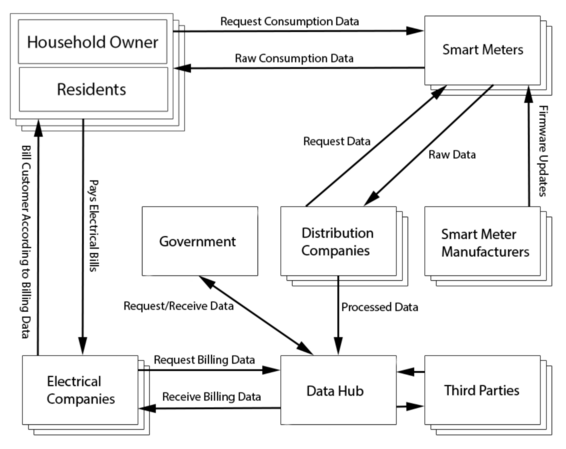
\includegraphics[width=\textwidth]{system}
  \caption{The smart meter system\cite{tdlm}}
  \label{contextual:system}
\end{figure}

As no fully implemented smart meter systems currently exist, a lot of assumptions will have to be made before it is possible to imagine how such a system could be attacked.
We do this in two steps.

The first step taken is to outline the system as closely as possible.
Since there is no single correct system architecture, we have chosen the one opted by our native country: Denmark.
This system outline is based on the sources and information gained in the previous sections.

The second step is to choose a segment of this system, which will function as our context model, on which our attack trees will ``carry out attacks''.

\subsection{The Smart Meter System}
The system is pictured in \cref{contextual:system}.
The lines indicate information flow between actors in the system.
The consumer (\textit{Household Owner/Residents}) can interact with the smart meter in order to control smart appliances and monitor the production of his home production devices.
The \textit{Data Hub} stores the consumption data of the consumer.
This data is available for the consumer, the \textit{Distribution Companies} and the \textit{Electrical Company}.
These three actors have permission to see the consumption data in different granularities.
The consumer can see the data in the finest granularity, whereas the distribution companies and the electrical companies has access to a coarser granularity that makes it possible for them to calculate the bill.

\textbf{Note:} The electrical companies send price information to the data hub (not pictured), which the consumer can see through the smart meter.

\subsection{Actors and threats}
Placing a smart meter in a consumers home and simultaneously requiring external access to its data is a complicated task with many potential risks.
\Cref{contextual:sm_model} represents this context and the actors therein.
This has been used as a starting point for a brainstorm that maps the potential attacks on the system.

The actors represented in \cref{contextual:sm_model} are not representative of the complete set of actors having some interaction with the system.
However these other actors communicate with the system through the smart meter and to not clutter the visual representation they have not been included.
They will still be listed as actors below and possible threats to/from them will be considered.

\begin{figure}[h]
  \centering
  \tikzstyle{man}=[font={\Gentsroom}, scale=5]
\tikzstyle{woman}=[font={\Ladiesroom}, scale=5]

\begin{tikzpicture}[every node/.style={inner sep=0,outer sep=0}, arrows={[round]}]

\draw (-5.5,6) rectangle (2,-0.5);
\node at (-1,5.5) {Household};

\draw  (-6.5,7) [fill=white] rectangle (-4,5.5) node[pos=.5,align=center] {Home\\Production};
\draw  (-5,1.5) [fill=white] rectangle (-3.5,0) node[pos=.5,align=center] {Smart\\Meter};
\draw  (-3,4.5) [fill=white] rectangle (-1,3) node[pos=.5,align=center] {Smart\\Appliance};
\draw  (-0.5,2) [fill=white] rectangle (0.5,1) node[pos=.5,align=center] {Client};
\draw  (-9,2.5) [fill=white] rectangle (-6.5,1) node[pos=.5,align=center] {Data Hub};

\node[man] (consumer) at (1,1) {};
\node [below=0.2 of consumer] {Consumer};

\node[man] (burglar) at (-6.5,0) {};
\node [below=0.2 of burglar] {Burglar};

\node[man] (external) at (3.5,5) {};
\node [below=0.2 of external] {External};

\node[man] (power) at (-7.5,6.5) {};
\node [below=0.2 of power,align=center] {Electrical\\Company};

\node[man] (distribution) at (-7.5,4) {};
\node [below=0.2 of distribution] {Distribution};

\node[woman] (partner) at (1,4) {};
\node [below=0.2 of partner] {Partner};

\node[man] (neighbour) at (3.5,0.5) {};
\node [below=0.2 of neighbour] {Neighbour};

\draw[dashed] (-4.5,5.5) -- (-4.5,1.5);
\draw[dashed] (-6.5,1.5) -- (-6,1.5) -- (-6,1) -- (-5,1);
\draw[dashed] (-3.5,1) -- (-2.5,1) -- (-2.5,1.5) -- (-0.5,1.5);
\draw[dashed] (-2.5,3) -- (-2.5,2.25) -- (-4,2.25) -- (-4,1.5);

\end{tikzpicture}
  \caption{The smart meter context model}
  \label{contextual:sm_model}
\end{figure}

\paragraph{Actors}\label{contextActors}
Below is the list of the actors represented in the full system and context.
As noted above, some of these actors are not represented visually in \cref{contextual:sm_model} but are part of the information flow of the entire system (see \cref{contextual:system}).
The list below will not describe the potential threats in the system, but only list the possible actors involved in such threats.
\begin{itemize}
\item \textbf{Consumer}\\
The resident of the depicted home and the one which power consumption is monitored.
The smart meter is installed in the consumers home.
The consumer may want to attack his own smart meter in order to reduce his power bill.
\item \textbf{Burglar}\\ A burglar can use the smart meter to find out when the consumer is home in order to break in as well as find out what products the consumer owns in order to assess him as a target.
\item \textbf{Neighbour}\\
The next door neighbour to the consumer.
We assume that the neighbour will perform attacks on the consumer in order to remove annoyances, such as loud appliances or music.
In case of neighbourly disputes, messing with the SM and connected appliances could also be viable strikes.
\item \textbf{Partner}\\
The consumer's partner.
It is assumed that this is not a person that is living with the consumer.
The partner would like to surveil or get revenge over the consumer in case of misdoings on the consumer's part, such as adultery.

\item \textbf{Electrical Company}\\
The company billing the consumer for his power consumption.
\item \textbf{Distribution Company}\\
Manages the part of the grid closest to the consumer and provides him with electricity.
Installs the smart meters in the consumers home.
\item \textbf{External}
\begin{itemize}
\item \textbf{Information gatherers}\\ 
Some companies depend on information of consumers and can use the information provided by the smart meter to profile consumers.
\item \textbf{Developers of third party apps}\\
The developer of apps that the consumer will use for monitoring his electrical consumption. Can be both mobile, desktop and web applications.
\item \textbf{Appliance company}\\ The provider of home appliances that can connect with the SM.
\item \textbf{Government}\\
The government officials (including counties and municipalities).
\item \textbf{States}\\ In countries with tension between them, one country could have an interest in attacking citizens of the opposing country.
\item \textbf{A terrorist organisation}\\ Terrorists can abuse the smart meter for terrorist acts, like shutting off power in a city or region.
\item \textbf{Environmental activists}\\ Activists can abuse the smart meter as a means of demonstrating environmental politics.
\item \textbf{Blackmailer}\\ A criminal who switches off all or some smart meters from an electrical company and demands money for switching them on again.
\end{itemize}
\end{itemize}

\paragraph{Objects}
\begin{itemize}
\item \textbf{Smart meter}\\ Controls home appliances and also records consumption for each.
\item \textbf{Appliance}\\ Has an option to be controlled from the smart meter. For instance a washing machine can be started and stopped when scheduled.
\end{itemize}

\subparagraph{Smart Meter}
The following describes the conceptual smart meter we have used in our considerations, based on \cref{background}, \citet{tdlm} and \citet{smart_meter_survey}.
The smart meter is installed in the household of the consumer, in this case a house.
Home appliances are connected to the SM and can be managed from it.
The SM can be accessed through an API.
The consumer can access and manage his home appliances connected to the smart meter through some sort of program for instance an app, developed by a third party.
The smart meter manufacturer has the ability to update software.
The electrical companies have the ability to get switch off the smart meter and get billing information from the smart meter.
The home appliance company can update the firmware of their appliances through the SM.
The smart meter sends its consumption data to the datahub.
Home production of electricity, for instance a windmill, is also connected to the smart meter.
